\section{Simulation Results}\label{sec:results}

The proposed method was implemented in C++ and tested using a \SI[mode=text]{3.20}{\GHz} CPU with
\SI{8}{GB} memory.  We demonstrate the results using three real-life assays and three randomly generated assays. The information of these test cases is shown in Table~\ref{tb_test}, where CPA (Colorimetric Protein Assay), IVD (In-Vitro Diagnostics) and PCR (Polymerase Chain Reaction) are real-world assays and the other three assays are randomly generated. The column $|O|$ in Table~\ref{tb_test} shows the number of operations in each assay. In the experiments, we used Gurobi \cite{gurobi} to solve the optimization problems.

The result of scheduling with storage minimization is shown in the columns $\boldsymbol{c_t}$, $\boldsymbol{t^E}$ and $\boldsymbol{t_s}$ in Table~\ref{tb_test}, where $\boldsymbol{c_t}$ is the fluid-storage times in flow channels, $\boldsymbol{t^E}$ is the execution time of the assay defined in (\ref{eq:latest_finishing}), and $\boldsymbol{t_s}$ is the runtime for solving the optimization problem (\ref{eq:minobj})--(\ref{eq:op_cond}), which was limited to 30 minutes for the solver to return the best-effort results. In architectural synthesis, we use a connection
grid to determine device locations and channel segments connecting them. The size of the grid is shown in
column $\boldsymbol{G}$ in Table~\ref{tb_test}. After architectural synthesis, the numbers of
edges (channel segments) and valves in the chip architecture are shown in the columns $\boldsymbol{n_e}$ and $\boldsymbol{n_v}$, respectively. Note the valves counted in the experiments do not include those built in mixers. The runtimes to generate chip architectures are shown in the column $\boldsymbol{t_r}$.

\begin{figure}[t]
    \centering
    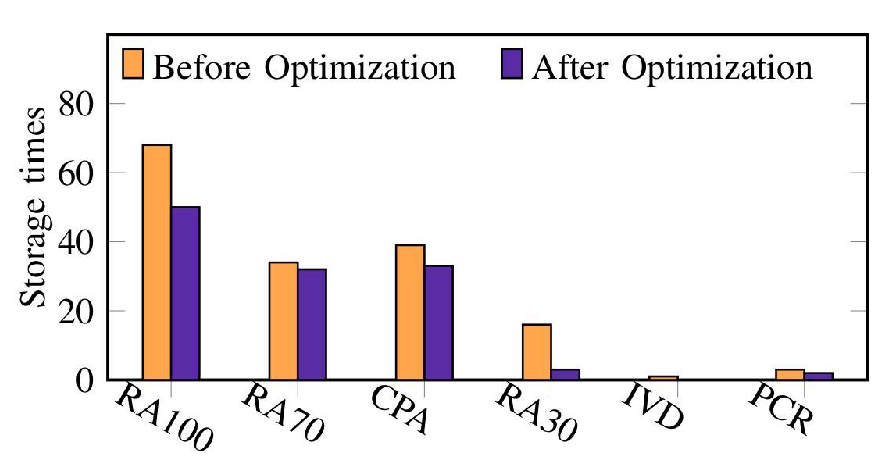
\includegraphics[width=0.85\linewidth]{Visio/storage_cmp.pdf}
  \caption{Comparison of storage times with and without storage optimization.}
      \label{fig:storage_cmp}
%\vspace{-0.5cm}
\end{figure}

\begin{figure}[t]
{\figurefontsize
\centering
\input{Fig/ideal_cmp.pdf_tex}
\caption{Comparison of the results with and without storage optimization.}
\label{fig:ideal_cmp}
}
\end{figure}

After completing the architectural synthesis, a certain biochip architecture with minimized total cost is generated. Then transportation tasks specified in the scheduling are mapped to the chip, so that certain flow paths can be constructed to realize the transportation network without any conflict. Note that extra channel segments and resources may be introduced to the chip by the proposed genetic algorithm if the existing on-chip resources are not sufficient to eliminate all the transportation conflicts. The corresponding results of flow-path planning are also shown in Table~\ref{tb_test}, where the columns $\boldsymbol{n_c}$ and $\boldsymbol{n_t}$ are the numbers of chromosomes and iterations used in the genetic algorithm, respectively. The total numbers of transportation-task groups generated after performing the sweepline algorithm are shown in the column $\boldsymbol{n_g}$. Inside each group, when mapping the transportation tasks to the biochip, their corresponding flow paths may conflict with each other, leading to a conflicting group. Accordingly, the numbers of conflicting transportation-task groups are shown in the column $\boldsymbol{n_{cg}}$. Note that all the aforementioned transportation conflicts are eliminated successfully after implementing the proposed adjustment strategies. Since introducing extra resources can further lead to more valves, the total number of valves in the chip after performing the architectural adjustment is shown in the column $\boldsymbol{n_{tv}}$. Moreover, the numbers of deadlocks occurred during the flow-path planning are shown in the column $\boldsymbol{d_{k}}$, and all these deadlocks can be removed by solving the ILP model defined in Section~\ref{sec:res_storage_deadlock}. The final execution time of the assay is shown in the column $\boldsymbol{t^{E'}}$, which is a little bit longer than the one shown in the column $\boldsymbol{t^{E}}$ due to the effects of the proposed scheduling adjustment method. Finally, the runtimes of the flow-path planning are shown in the column $\boldsymbol{t_p}$, which are acceptable for a high-quality transportation network without any conflict.

%In the iterative physical design step, the result of architectural synthesis was first scaled with the unit equal to the minimum channel distance specified by the designer. Afterwards, devices were inserted to nodes determined by architectural synthesis and the layout was iteratively compressed to reduce chip area. The physical dimensions of the chip after architectural synthesis, after device insertion and after iterative compression are shown in the columns $\boldsymbol{d_r}$, $\boldsymbol{d_e}$ and $\boldsymbol{d_p}$, respectively. Since the output of architectural synthesis was already planar, the proposed iterative layout compression can reduce the chip area effectively. The runtime of the physical design  phase is shown in the $\boldsymbol{t_p}$ column, which is also acceptable for layout generation.

\pgfplotsset{compat=1.3,
    /pgfplots/ybar legend/.style={
    /pgfplots/legend image code/.code={%
       \draw[##1,/tikz/.cd,yshift=-0.25em]
        (0cm,0cm) rectangle (5pt,0.8em);},
   }
}

We also evaluated the effectiveness of the proposed storage optimization in scheduling
and architectural synthesis. \figname~\ref{fig:storage_cmp} shows the comparison results on storage times. It can be seen that the storage requirements in each assay are reduced significantly after applying the proposed optimization method.  Moreover, \figname~\ref{fig:ideal_cmp} shows the comparison of execution time of assays,
the number of edges and the number of valves in the two cases with and without
storage optimization.
In this comparison, it can be observed that storage optimization
generated comparable execution time in the cases IVD and PCR, but the execution
time of RA30 is slightly longer, which is acceptable for most biochemical
experiments. However, the numbers of edges and valves in the result
of RA30 are much smaller, because storage optimization
improves the efficiency of channels and thus valves effectively so that fewer
resources are required to execute the assays.

\begin{figure}[t]
{\figurefontsize
\centering
\vskip 5pt
\begin{tikzpicture}
\begin{axis}[
x=1.1cm, y=0.27cm, ymax=12, line width=0.75pt,
ylabel={Channel (Valve) Ratio}, ylabel shift=-6pt, 
xtick={1,...,6},xticklabels={RA100, RA70, CPA, RA30, IVD, PCR},
x tick label style={rotate=330, xshift=-15pt,yshift=-5pt,anchor=west}, 
xticklabel pos=left, xtick align=outside, xtick pos=left,
ytickmin=0,ytickmax=10, 
ytick={0,5,10}, yticklabels={0,0.5,1},
legend columns=2, legend style={at={(0.5,0.9)}, anchor=center, nodes={inner xsep=2pt},
draw=none, column sep=1pt},
ybar=0pt, bar width=7
]
   \addplot[line width=0.5pt, black, fill=orange!70!white] table[x=cir,y=edge] 
{edge_valve_percentage.dat};
   \addplot[line width=0.5pt, black, fill=blue!65!orange] table[x=cir,y=valve] 
{edge_valve_percentage.dat};

   \legend{Channel\hspace*{8pt}, Valve\hspace*{8pt}}
\end{axis}
\end{tikzpicture}

%\begin{tikzpicture}
\begin{axis}[
x=1.1cm, y=0.27cm, ymax=12, line width=0.75pt,
ylabel={Channel (Valve) Ratio}, ylabel shift=-6pt, 
xtick={1,...,6},xticklabels={RA100, RA70, CPA, RA30, IVD, PCR},
x tick label style={rotate=330, xshift=-15pt,yshift=-5pt,anchor=west}, 
xticklabel pos=left, xtick align=outside, xtick pos=left,
ytickmin=0,ytickmax=10, 
ytick={0,5,10}, yticklabels={0,0.5,1},
legend columns=2, legend style={at={(0.5,0.9)}, anchor=center, nodes={inner xsep=2pt},
draw=none, column sep=1pt},
ybar=0pt, bar width=7
]
   \addplot[line width=0.5pt, black, fill=orange!70!white] table[x=cir,y=edge] 
{edge_valve_percentage.dat};
   \addplot[line width=0.5pt, black, fill=blue!65!orange] table[x=cir,y=valve] 
{edge_valve_percentage.dat};

   \legend{Channel\hspace*{8pt}, Valve\hspace*{8pt}}
\end{axis}
\end{tikzpicture}

\caption{
Edge and valve ratios in the result of
architectural synthesis compared with the original edges and valves
in the connection grid.}
\label{fig:edge_valve_percentage}
}
\end{figure}

\begin{figure}[t]
{\figurefontsize
\centering
\begin{tikzpicture}
\begin{axis}[
x=1.1cm, y=0.26cm, ymax=12, line width=0.75pt,
ylabel={Exec./Valve Ratio}, ylabel shift=-6pt, 
xtick={1,...,6},xticklabels={RA100, RA70, CPA, RA30, IVD, PCR},
x tick label style={rotate=330, xshift=-15pt,yshift=-5pt,anchor=west}, 
xticklabel pos=left, xtick align=outside, xtick pos=left,
ytickmin=0,ytickmax=10, 
ytick={0,5,10}, yticklabels={0,0.5,1},
legend columns=2, legend style={at={(0.5,0.9)}, anchor=center, nodes={inner xsep=2pt},
draw=none, column sep=1pt},
ybar=0pt, bar width=7
]
   \addplot[line width=0.5pt, black, fill=orange!70!white]
table[x=cir,y=exetime] 
{exe_time_valve_cmp.dat};
   \addplot[line width=0.5pt, black, fill=blue!65!orange] table[x=cir,y=valve] 
{exe_time_valve_cmp.dat};
   \legend{Execution Time\hspace*{9pt}, Valve\hspace*{8pt}}
\end{axis}
\end{tikzpicture}

%\begin{tikzpicture}
\begin{axis}[
x=1.1cm, y=0.26cm, ymax=12, line width=0.75pt,
ylabel={Exec./Valve Ratio}, ylabel shift=-6pt, 
xtick={1,...,6},xticklabels={RA100, RA70, CPA, RA30, IVD, PCR},
x tick label style={rotate=330, xshift=-15pt,yshift=-5pt,anchor=west}, 
xticklabel pos=left, xtick align=outside, xtick pos=left,
ytickmin=0,ytickmax=10, 
ytick={0,5,10}, yticklabels={0,0.5,1},
legend columns=2, legend style={at={(0.5,0.9)}, anchor=center, nodes={inner xsep=2pt},
draw=none, column sep=1pt},
ybar=0pt, bar width=7
]
   \addplot[line width=0.5pt, black, fill=orange!70!white]
table[x=cir,y=exetime] 
{exe_time_valve_cmp.dat};
   \addplot[line width=0.5pt, black, fill=blue!65!orange] table[x=cir,y=valve] 
{exe_time_valve_cmp.dat};
   \legend{Execution Time\hspace*{9pt}, Valve\hspace*{8pt}}
\end{axis}
\end{tikzpicture}

\caption{Comparison of execution time and the number of valves
in the results with channel caching and dedicated storage unit.}
\label{fig:exe_time_valve_cmp}
}
\end{figure}

\begin{figure}[t]
{
  \figurefontsize
\centering
%\vskip 5pt
\pgfplotsset{compat=1.3,
    %legend drawing style, single bar instead of the default double mini bars
    /pgfplots/ybar legend/.append style={ 
        /pgfplots/legend image code/.code={%
           \draw[##1,/tikz/.cd,yshift=-0.25em]
           (0cm,0cm) rectangle (5pt,0.8em);
        },
    }
}

%%sharp linear plots
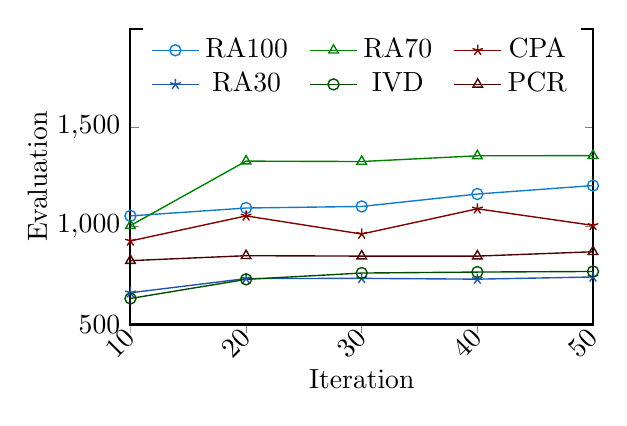
\begin{tikzpicture}
%remove space surrounding text nodes and the whole picture caused by text
%[every node/.style={inner sep=0,outer sep=0}]

%\pgfplotstableread{
%Iteration IVD\_IVD      
%1       99.69	   
%2       99.59	   
%3       99.58	  
%4       99.80	   
%5       99.85	   
%6       99.11	   
%7       87.73	   
%8       99.83	  
%9       99.42
%10      99.68
%}\loadedtable

\pgfplotstableread{
Iteration RA100 RA70	CPA	RA30	IVD	PCR
1	1051	1002	924	661	632	824
2	1091	1329	1051	733	729	849
3	1099	1327	959	734	761	847
4	1162	1356	1087	730	766	847
5	1205	1357	1003	741	769	869

}\loadedtable

\begin{axis}[
%xaxis styles
%xticklabels={s5378,s9234, s13207, s15850, s38584,systemcdes, mem\_ctrl, usb\_funct, ac97\_ctr, pci\_bridge32}, 
xticklabels={10, 20, 30, 40, 50},
xtick={1,...,5},
%x axis limits
xmin=1, xmax=5,
%x and y axes scaling
x=1.4685714cm, y=0.0025cm, 
x tick label style={rotate=45, xshift=0pt,yshift=0pt,anchor=east, 
%"inner sep" removes the space surrounding label tick texts at the bottom,
%so that there is no useless white space at the lower boundary of the picture. The
%space of tick label texts need to be removed because they are the lowest
%units without an xlable
inner sep=0}, 
xticklabel pos=left, xtick align=outside, xtick pos=left,
%
%y axis limits
ymin=500, ymax=2000, 
%yaxis styles
ylabel={Evaluation}, 
xlabel={Iteration}, 
%"inner sep" for ylabel removes the white space on the leftmost edge of the picture
ylabel style={inner sep=0}, 
ylabel shift=0pt, ytickmin=500,ytickmax=1500, 
% ytick = {700,800,900,1000,1100,1200,1300}, yticklables = {700,800,900,1000,1100,1200,1300}
%
%legend styles
legend columns=3, 
legend style={
at={(0.5,0.87)}, anchor=center, 
%column separation between legend items
/tikz/every even column/.append style={column sep=0.2cm},
%distance between legend symbols and text nodes
%column sep=2.5cm,
%space surrounding the text boxes in legend
%nodes={inner xsep=20pt},
%no stroke in legend
draw=none, 
},
%
%axis drawing line width
line width=0.75pt,
major tick length=3pt,
]  \addplot[sharp plot, line width=0.5pt, cyan!60!blue, mark=o, fill=none] table[x=Iteration,y=RA100] {\loadedtable};
\addplot[sharp plot, line width=0.5pt, green!50!black, mark=triangle, fill=none] table[x=Iteration,y=RA70] {\loadedtable};
\addplot[sharp plot, line width=0.5pt, red!50!black, mark=star, fill=none] table[x=Iteration,y=CPA] {\loadedtable};
\addplot[sharp plot, line width=0.5pt, cyan!30!blue, mark=star, fill=none] table[x=Iteration,y=RA30] {\loadedtable};
\addplot[sharp plot, line width=0.5pt, green!30!black, mark=o, fill=none] table[x=Iteration,y=IVD] {\loadedtable};
\addplot[sharp plot, line width=0.5pt, red!30!black, mark=triangle, fill=none] table[x=Iteration,y=PCR] {\loadedtable};
   %\addplot[sharp plot, line width=0.5pt, green!50!black, mark=triangle, fill=none] table[x=Iteration,y=tested] {\loadedtable};
   %\addplot[sharp plot, line width=0.5pt, red!50!black, mark=star, fill=none] table[x=Iteration,y=nobuffer] {\loadedtable};
\legend{RA100,RA70,CPA,RA30,IVD,PCR}
\end{axis}
\end{tikzpicture}

%\begin{tikzpicture}
\begin{axis}[
x=1.1cm, y=0.27cm, ymax=12, line width=0.75pt,
ylabel={Channel (Valve) Ratio}, ylabel shift=-6pt, 
xtick={1,...,6},xticklabels={RA100, RA70, CPA, RA30, IVD, PCR},
x tick label style={rotate=330, xshift=-15pt,yshift=-5pt,anchor=west}, 
xticklabel pos=left, xtick align=outside, xtick pos=left,
ytickmin=0,ytickmax=10, 
ytick={0,5,10}, yticklabels={0,0.5,1},
legend columns=2, legend style={at={(0.5,0.9)}, anchor=center, nodes={inner xsep=2pt},
draw=none, column sep=1pt},
ybar=0pt, bar width=7
]
   \addplot[line width=0.5pt, black, fill=orange!70!white] table[x=cir,y=edge] 
{edge_valve_percentage.dat};
   \addplot[line width=0.5pt, black, fill=blue!65!orange] table[x=cir,y=valve] 
{edge_valve_percentage.dat};

   \legend{Channel\hspace*{8pt}, Valve\hspace*{8pt}}
\end{axis}
\end{tikzpicture}

\caption{Average convergence curves of the proposed genetic algorithm.}
\label{fig:iteration}
}
\end{figure}

\begin{figure}[t]
    \centering
    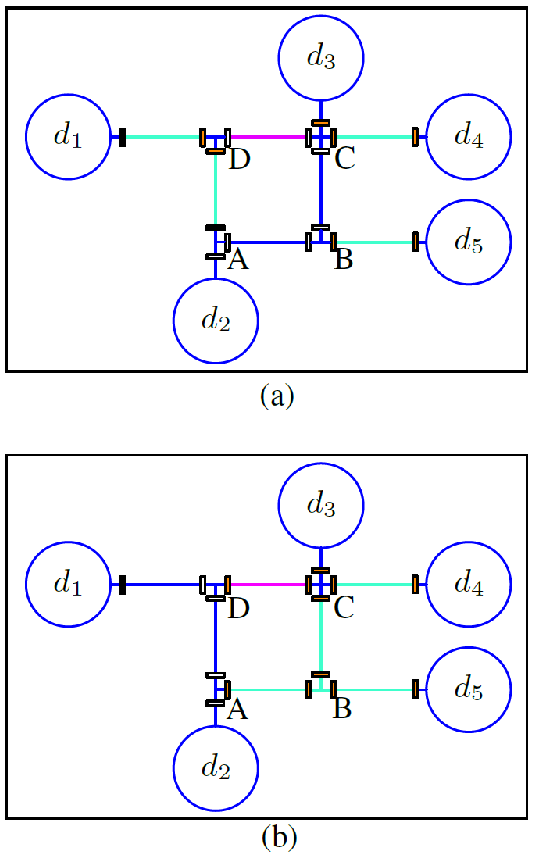
\includegraphics[width=0.6\linewidth]{Visio/RA30_exe_flow.pdf}
    %\input{Fig/RA30_exe_flow.pdf_tex}
  \caption{Snapshots of the synthesized chip executing RA30 at (a) 35 s and (b) 45 s. The channel segments in blue are transporting and in purple are caching fluid samples.}
      \label{fig:RA30_exe_1}
%\vspace{-0.5cm}
\end{figure}

\begin{figure}[t]
    \centering
    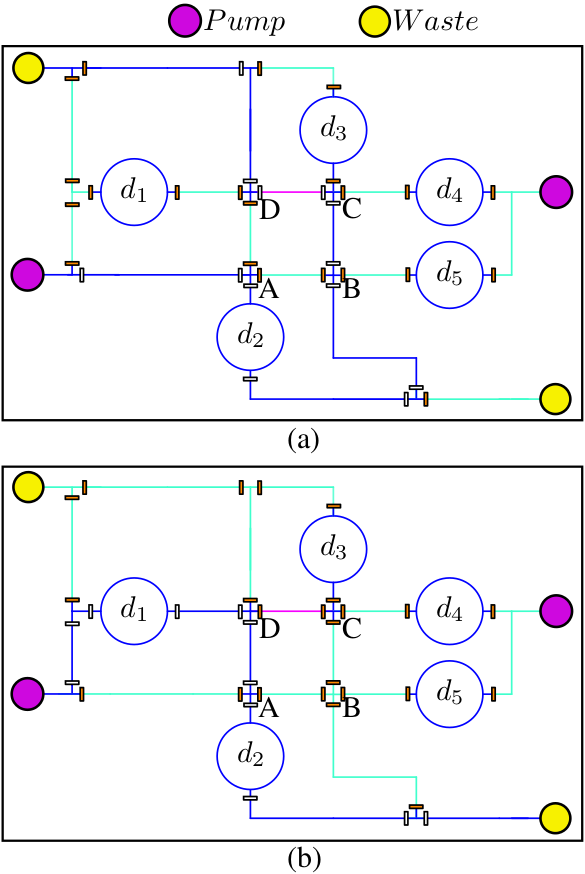
\includegraphics[width=0.7\linewidth]{Visio/RA30_exe_flow_test.png}
    %\input{Fig/RA30_exe_flow_test.pdf_tex}
  \caption{Snapshots of the synthesized chip executing RA30 with constructed flow paths at (a) 35 s and (b) 45 s. The channel segments in blue are transporting and in purple are caching fluid samples.}
      \label{fig:RA30_exe_2}
%\vspace{-0.5cm}
\end{figure}

In architectural synthesis, we start with a connection grid. After synthesis, only the edges that are used at least once are kept in the result. The ratios of the number of used edges to the total number of all the edges in the grid is shown in \figname~\ref{fig:edge_valve_percentage}, where all these ratios are smaller than 1, and a half of them are even close to 0, showing that the architectural synthesis approach confines resource usage effectively on only a part of edges to reduce resource usage.  After removing the unused edges, the number of valves is also reduced, as shown by the valve ratios in \figname~\ref{fig:edge_valve_percentage}.
% \begin{figure}[t]
%      \centering
%      \input{Fig/RA30_exe_flow_test.pdf_tex}
%    \caption{Snapshots of the synthesized chip executing RA30 with constructed flow paths at (a) 35 s and (b) 45 s. The channel segments in blue are transporting and in purple are caching fluid samples.}
%        \label{fig:RA30_exe_2}
%  %\vspace{-0.5cm}
% \end{figure}

% \begin{figure}[t]
%   {\figurefontsize
%   \centering
%   \input{Fig/RA30_exe_flow_test.pdf_tex}
%   \caption{Comparison of the results with and without storage optimization.}
%   \label{fig:ideal_cmp}
%   }
%   \end{figure}


In previous methods, the storage and caching problem has not been considered.
When there is a storage requirement, it is usually assumed that
the intermediate fluid sample is transported to a dedicated storage unit.
To compare the efficiency of the synthesized chip architecture with that from
the assumed storage transportation, we examine the storage requirement in the
schedules generated by the
proposed method. When storage requirements appear, they are assumed to queue
at the
entrance of a dedicated storage unit.
%and stored after traveling through the multiplexer-style port.
The maximum size of the storage cells is the
maximum number of fluid samples stored simultaneously in the storage unit.
Due to the bandwidth limit of
the storage unit, the execution of the assay is thus prolonged. In addition,
the dedicated storage unit used many valves to control the access of storage
cells.
%leading to even more valves.
Channel segments and
valves in the result from the proposed method and the result with a dedicated
storage unit is shown in \figname~\ref{fig:exe_time_valve_cmp}. From this
comparison,
it can be seen that the execution time
and the number of valves are well below 1,
leading to a more efficient execution of the assay with fewer resources.
%For example, the execution time reduction for RA100 has already reached about 28\%.
% is made possible by the proposed method.




%15 gid=3000000
15 uid=3603518
27 mtime=1539610141.357741
27 ctime=1539610141.358741
27 atime=1539610141.360739


Moreover, in the flow-path planning stage, since the proposed genetic algorithm plays an important role in determining the new biochip architecture, to evaluate its efficiency, Fig.~\ref{fig:iteration} illustrates the corresponding convergence curves with respect to different bioassays. It can be seen that the average fitness level of the population is improved as iteration time increases, and the proposed algorithm reaches a convergence quickly in most of the test cases. Note that since the genetic algorithm works in a random manner, stochastic fluctuations may occur during iterations, leading to an unstable region in the convergence curve of the assay ``CPA", but our algorithm can still find a feasible flow-path planning solution for this assay.





%We also tested how different ports number on a biochip will affect the resource usage and assay execution time. The Fig.~\ref{fig:port_valve_number} compares the valve numbers in the final synthesis results when given 4,6 and 8 ports. Half of the ports are pump ports and the other half are waste ports. As the histogram shows, the more ports are connected to an architecture, the less valves needed in the final synthesis results to enable constructing flow paths. The Fig. ~\ref{fig:port_exe_time} compares assay executing time with different port number. As we can see, the port number makes little difference on the assay execution time. This is because when optimizing resource usage and assay execution time at the same time, optimizing resource usage is given more weight.

%\begin{figure}[t]
%{\figurefontsize
%\centering
%\begin{tikzpicture}
\begin{axis}[
% x=1.1cm, y=0.25cm, ymax=12, line width=0.75pt,
x=1.1cm, y=0.60, ymax=150, line width=0.75pt,
ylabel={Valve Number}, ylabel shift=-6pt, 
xtick={1,...,6},xticklabels={RA100, RA70, CPA, RA30, IVD, PCR},
x tick label style={rotate=330, xshift=-15pt,yshift=-5pt,anchor=west}, 
xticklabel pos=left, xtick align=outside, xtick pos=left,
ytickmin=0,ytickmax=120,
% ymin = 0,
% ymax = 1,
ytick={0,20,40,60,80,100,120}, yticklabels={0,20,40,60,80,100,120},
legend columns=3, legend style={at={(0.5,0.9)}, anchor=center, nodes={inner xsep=2pt},
draw=none, column sep=1pt},
ybar=0pt, bar width=7
]

   \addplot[line width=0.5pt, black, fill=orange!70!white] table[x=cir,y=edge] 
{port_valve_number.dat};
   \addplot[line width=0.5pt, black, fill=blue!65!orange] table[x=cir,y=valve] 
{port_valve_number.dat};
   \addplot[line width=0.5pt, black, fill=blue!40!orange] table[x=cir,y=valve2] 
{port_valve_number.dat};
   \legend{4 Ports\hspace*{0.5pt}, 6 Ports\hspace*{0.5pt},8 Ports\hspace*{0.5pt}}
\end{axis}
\end{tikzpicture}

%\caption{Comparison of numbers of valve needed of architectures with different port number.}
%\label{fig:port_valve_number}
%}
%\end{figure}

%\begin{figure}[t]
%{\figurefontsize
%\centering
%\begin{tikzpicture}
\begin{axis}[
% x=1.1cm, y=0.25cm, ymax=12, line width=0.75pt,
x=1.1cm, y=1cm, ymax=3, line width=0.75pt,
ylabel={Assay Execution Time}, ylabel shift=-6pt, 
xtick={1,...,6},xticklabels={RA100, RA70, CPA, RA30, IVD, PCR},
x tick label style={rotate=330, xshift=-15pt,yshift=-5pt,anchor=west}, 
xticklabel pos=left, xtick align=outside, xtick pos=left,
ytickmin=0,ytickmax=3,
% ymin = 0,
% ymax = 1,
ytick={0,0.5,1.0,1.5,2.0,2.5}, yticklabels={0,500,1000,1500,2000,2500},
legend columns=3, legend style={at={(0.5,0.9)}, anchor=center, nodes={inner xsep=2pt},
draw=none, column sep=1pt},
ybar=0pt, bar width=7
]

   \addplot[line width=0.5pt, black, fill=orange!70!white] table[x=cir,y=edge] 
{port_exe_time.dat};
   \addplot[line width=0.5pt, black, fill=blue!65!orange] table[x=cir,y=valve] 
{port_exe_time.dat};
   \addplot[line width=0.5pt, black, fill=blue!40!orange] table[x=cir,y=valve2] 
{port_exe_time.dat};
   \legend{4 Ports\hspace*{1pt}, 6 Ports\hspace*{1pt},8 Ports\hspace*{1pt}}
\end{axis}
\end{tikzpicture}

%\caption{Comparison of assay execution time of  architectures with different port number.}
%\label{fig:port_exe_time}
%}
%\end{figure}

Finally, we show the execution snapshots of the assay RA30
in \figname~\ref{fig:RA30_exe_1} and \figname~\ref{fig:RA30_exe_2}, respectively.
\figname~\ref{fig:RA30_exe_1} demonstrates the fluid transportation without considering the actual flow paths construction. In \figname~\ref{fig:RA30_exe_1}(a), a transportation path is formed as $d_2\to A\to B \to C \to D $ to store a fluid sample into the channel segment between $C$ and $D$. In \figname~\ref{fig:RA30_exe_1}(b), a transportation path is constructed as $d_1\to D \to A \to d_2$ while the channel segment between $C$ and $D$ is caching a fluid sample.
\figname~\ref{fig:RA30_exe_2} demonstrates the fluid transportation on the chip architecture after completing the flow-path palnning. In \figname~\ref{fig:RA30_exe_2}(a), a flow path is
formed as $pump \to A \to d_2\to B \to C \to D\to waste$ to store a fluid sample
into the channel segment between $C$ and $D$. In \figname~\ref{fig:RA30_exe_2}(b), a flow path is formed as $pump
\to d_1 \to D \to A \to d_2 \to waste$, while an intermediate liquid is stored between $C$ and $D$.



%a flow path is formed as pump �� a��d2��b��c��d��waste����д���ˣ�ʵ�ڱ�Ǹ��


